\section{Concept generation}
	With all the premise that lead the development of the project, the first thing that has to be done is generate the concept that can later be compared to choose the best design solution that can become a concrete realization of the ideas.
	
	\paragraph{Kinematic configurations} The first key operation that the robot has to perform is reaching a desired point on the working space and so, in planar kinematics, the machine should present two degrees of freedom that allow to reach all the possible positions; this can be done considering 3 main joint configuration that allows to perform such operations:
	\begin{itemize}
		\item double prismatic joints (figure \ref{fig:kinematiccoupling}.a) where two perpendicular linear guides can be used to move on the plane;
		\item prismatic and revolute joint (figure \ref{fig:kinematiccoupling}.b) where the arm that's free to rotate it's mounted on top of a linear guide. This kind of kinematic chain is currently used by the MindsHub concept;
		\item double revolute joints (figure \ref{fig:kinematiccoupling}.c), typical configuration of a robot arm, that constraint the framing point to be fixed.
	\end{itemize}
	
	\begin{figure}[bht]
	\centering
		\begin{subfigure}{0.32\linewidth}
			\centering 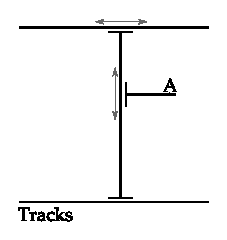
\includegraphics[width=4cm]{kinematics-prism-prism}
			\caption{}
		\end{subfigure}
		\begin{subfigure}{0.32\linewidth}
			\centering 
\includegraphics[width=4cm]{kinematics-prism-rot}
			\caption{}
		\end{subfigure}
		\begin{subfigure}{0.32\linewidth}
			\centering 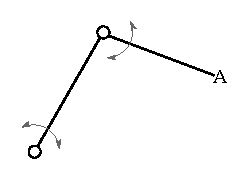
\includegraphics[width=4cm]{kinematics-rot-rot}
			\caption{}
		\end{subfigure}
		\caption{main kinematics coupling that allows to univocally determine the position of a point $A$ in a plane: (a) double prismatic joints, (b) prismatic and revolute joint, (c) double revolute joints.}
		\label{fig:kinematiccoupling}
	\end{figure}
	
	By a first analysis the third configuration (double revolute joint) isn't feasible for the project due to the fact that the system presents a fixed pivot point respect to the frame and to work more area it's mandatory to increase the length of the edges (and this is an issue for the \textit{extendibility} of the machine).
	
	\paragraph{Concept \#1} The first concept (figure \ref{fig:prot:1}) is realised with a double prismatic joint. In particular point $A$ and $A'$ relies on parallel tracks placed on the ground that can be extended in order to increase the cultivated area. The working arm can move along an elevated beam connecting the track (point $B$) and can move vertically to cultivate point $P$.
	
	\begin{figure}[bht]
		\centering 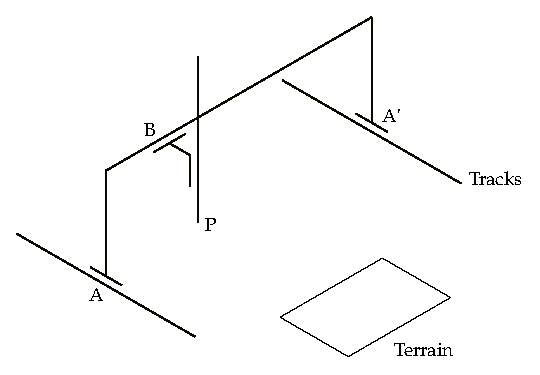
\includegraphics[width=8.5cm]{Prototype-1}
		\caption{concept \#1 realised with double prismatic joint.}
		\label{fig:prot:1}
	\end{figure}
	
	This structure present a frame for the arm that's stable while operating due to it's arch structure; possible problem to this implementation is that long elevated beam (subjected to the loads of the arms and it's mass) can deflect and fail statically. Also, if possible, rotoidal coupling should be used (and for this we can refer to concept \#2).
	
	\paragraph{Concept \#2}	The second concept (figure \ref{fig:prot:2}) is similar to the first one but one prismatic joint is replaced with a revolute connection put in the middle of the elevated beam. The length of the edge $BP$ from a top view must be equal to half the length of the supporting bar in order to reach all points in the rectangular space.

	\begin{figure}[bht]
		\centering 
\includegraphics[width=8.3cm]{Prototype-2}
		\caption{concept \#2 realised with a combination of both prismatic and revolute joint.}
		\label{fig:prot:2}
	\end{figure}
	
	This structure also presents the pro of concept \#1 of having a stable frame structure for the operating arm due to it's arch conformation and, as addition, uses a revolute joint to control the second degree of freedom of the arm. However this implementation increases the mechanical load on the elevated beam (increasing the torsion due to the higher arm of the actions on the tool tip respect to the elevated bar).
	
	\paragraph{Concept \#3}	The third concept (figure \ref{fig:prot:3}) is similar to \#2 but instead of using two parallel tracks, the prismatic joint uses only one of them.

	\begin{SCfigure}[1.5][bht]
		\centering 
\includegraphics[width=4.6cm]{Prototype-3}
		\caption{concept \#3  realised with a combination of both prismatic and revolute joint.}
		\label{fig:prot:3}
	\end{SCfigure}

	This implementation avoid the problem of high deflection of concepts \#1 and \#2 by removing the long elevated framing beam, but also increases the reactional momentum that the prismatic joint $A$ should bear in order to maintain stable the system.
	
	
\subsection{Decision matrix}
	With a brief overview of the 3 main concept generated, the unbiased choice can be performed by constructing and evaluating the decision matrix (table \ref{tab:decitionmatrix}). The main objective evaluated are:
	
	
\begin{sidewaystable}[p]
	\rule{\linewidth}{2pt}
	\caption{decision matrix.}
	\rule{\linewidth}{1pt} \vspace{0mm}	
	
	\begin{center}
		\begin{tabular}{p{4cm} c c | c c c | c c c | c c c}
			\multicolumn{3}{c}{} & \multicolumn{3}{c}{Concept \#1} & \multicolumn{3}{c}{Concept \#2} & \multicolumn{3}{c}{Concept \#3} \\
			Objective &  Weight & Parameter &
			Mag & Score & Value &
			Mag & Score & Value &
			Mag & Score & Value \\ \hline
			Material costs & 0.2 & relative \texteuro &
			medium & 7 & 1.4 &
			high & 5 & 1 & 
			low & 9 & 1.8 \\
			
			Reliability & 0.3 & experience &
			high & 9 & 2.7 &
			medium & 7 & 2.1 & 
			very low & 4 & 1.2 \\
			
			Crit \#3 & w \#3 & par \#3 &
			1a & 1b & 1c &
			2a & 2b & 2c & 
			3a & 3b & 3c \\
			
			Crit \#4 & w \#3 & par \#3 &
			1a & 1b & 1c &
			2a & 2b & 2c & 
			3a & 3b & 3c \\
			
			Crit \#5 & w \#5 & par \#5 &
			1a & 1b & 1c &
			2a & 2b & 2c & 
			3a & 3b & 3c \\
			
			
			
			\hline
			\multicolumn{3}{r|}{Overall score:} &&& 10 &&& 8 &&& 4
		\end{tabular}
	\end{center}
	
	\vspace{3mm}
	\rule{\linewidth}{1pt}
	{
		\scriptsize
		Other info
	}	
	
	\rule{\linewidth}{2pt}
	
\end{sidewaystable}
	
	\begin{itemize}
		\item costs: based on the estimated material cost considering quantity and types of parts that can be used for the implementation;
		\item reliability: expected mechanical  resistance of the structure subjected to nominal loads as well as unexpected external loads (such environment of customer that interact with the structure);
		
		\item lifetime: expected lifetime of the product based on fatigue considerations;
		
		\item adaptability: criteria that evaluates how easy is to modify geometrical parameters to meet specific custom requirement of the final customer based on asperity and tolerances of the terrain to cultivate;
		
		\item team experience: based on the overall design feasibility made by the team.
	\end{itemize}

	With the decision matrix completed the chosen concept is the first on which the motion is performed only by prismatic joints.
	
	
\subsection{Material selection}
	
	The main structural components are beams that, for client requirements, should be standard and so for this reason T slot extruded aluminium profiles (figure \ref{fig:tslot:crosssectionexample}) are chosen after the following considerations:
	\begin{itemize}
		\item better volume-to-price ratio and lower density (respect to inox steels), so reducing costs associated to the spare parts and shipping;
		\item availability in the marker: there are a lot of vendors that provide profiles with various geometrical dimensions, different aluminium alloy and surface finishes. This spare parts can be easily accessed by every private costumer;
		\item for T slot extruded profiles lots of auxiliary components (such supporting brackets, fasteners, hinges...)  are provided from the same profiles manufacturers, reducing the need of custom made part and so decreasing the costs.
	\end{itemize}

	This elements can be also purchased with an anodized finish that allows to improve the corrosion resistance and so increasing the expected life time of the product in uncontrolled outdoor environment.
	
	\begin{SCfigure}[1.5][bh]
		\centering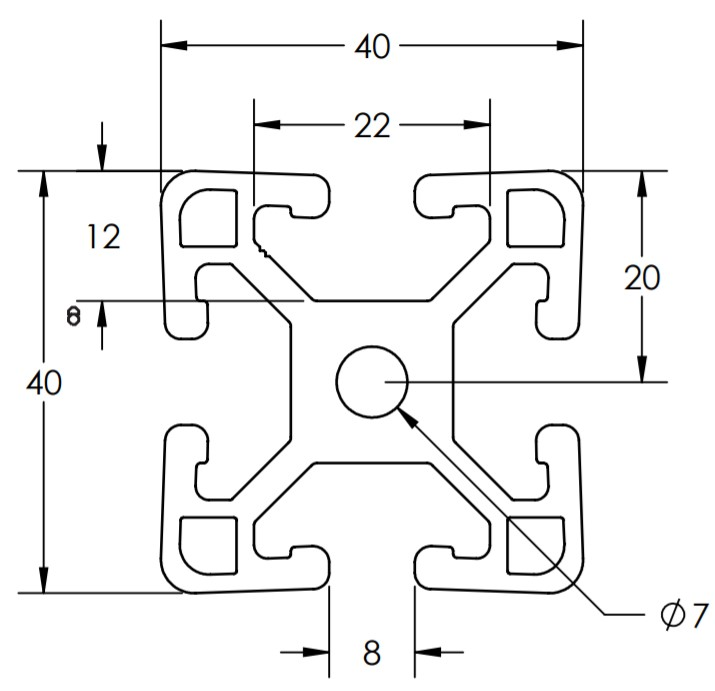
\includegraphics[width=5cm]{tslot-profile-example}
		\caption{technical drawing of a T-slot profile's cross-section. The particular sketch represent the model \texttt{TS40-40LM} by Tslots \cite{tslot-ds}.}
		\label{fig:tslot:crosssectionexample}
	\end{SCfigure}
	
	\paragraph{Mechanical properties} For the design part the following mechanical properties are considered: ultimate tensile strength $\sigma_{uts} = 260 MPa$, yielding strength $\sigma_{ys} = 240 MPa$, Young's module $E = 70 GPa$, Poisson's ratio $\nu = 0.32$; this are mean value and full material designation can be found on table \ref{tab:beammaterial} (page \pageref{tab:beammaterial}).\\
	For the final verification more detailed mechanical properties are going to be used depending on the final profile selection.
	
	
	
	
	
		
	
	
	
	
	
	
	
	
	
	
	
	
	
	
	
	
	
	
	
	
	
	
	
	
	
	
	
	
	
	
	
	
	
	
	
	
	
	
	
	
	
	
	
	
	
	
	
	
	
	
	
	
	
	
	
	
	
	
	